\documentclass[12pt]{article}
\usepackage{amssymb}
\usepackage{graphicx}
\usepackage{amsmath}
\usepackage[counterclockwise]{rotating}
\usepackage[hidelinks]{hyperref}
%\hypersetup{colorlinks,urlcolor=blue}
\hypersetup{colorlinks=true,citecolor=blue,pdfborder=000, urlcolor=red}
\usepackage{graphicx} % support the \includegraphics command and options
\usepackage[para,online,flushleft]{threeparttable}
\usepackage[round,semicolon]{natbib}  % This is for reference
\usepackage{cite}  % This is for reference
\usepackage{longtable}
%\usepackage{pdflscape}
\usepackage{rotating}
\usepackage{fancyhdr} % This should be set AFTER setting up the page geometry
\usepackage{epstopdf}
\usepackage{tikz}
\usepackage{caption}
\usepackage{subcaption}
\usepackage{natbib} %This code is for Mac
\usepackage{booktabs} % for much better looking tables
\usepackage{array} % for better arrays (eg matrices) in maths
%\usepackage{paralist} % very flexible & customisable lists (eg. enumerate/itemize, etc.)
\usepackage{verbatim} % adds environment for commenting out blocks of text & for better verbatim
%\usepackage{subfig} % make it possible to include more than one captioned figure/table in a single float
% These packages are all incorporated in the memoir class to one degree or another...
\renewcommand{\arraystretch}{1.0} % 將表格行間距加大為原來的 1.2 倍
%%% HEADERS & FOOTERS
\usepackage{fancyhdr} % This should be set AFTER setting up the page geometry
%\pagestyle{fancy} % options: empty , plain , fancy
\usepackage{float} % 可固定表的位置
\usepackage{lscape}
\usepackage{bookmark} % Allow customized pdf bookmark
\usepackage{tabularx}

\setcounter{MaxMatrixCols}{12}

\renewcommand{\baselinestretch}{1.0}
\usepackage{indentfirst}
\usepackage{setspace,caption}
\captionsetup{font=doublespacing}% Double-spaced float captions
\doublespacing% Double-spaced document text

\setlength{\topmargin}{-0.5in}
\setlength{\textheight}{8.8in}
\setlength{\evensidemargin}{0.0in}
\setlength{\oddsidemargin}{0.0in}
\setlength{\textwidth}{6.5in}
%\input{tcilatex}

%%%%%%%  Change to Times New Roman format
\usepackage[tmargin=1in,bmargin=1in,lmargin=1in,rmargin=1in]{geometry}
%\usepackage{fontspec}
%\usepackage{xcolor}
\usepackage{titlesec}
%\defaultfontfeatures{Ligatures=TeX}
% Set sans serif font to Arial
%\setsansfont{Arial}
% Set serifed font to Times New Roman
%\setmainfont{Times New Roman}
% Set formats for each heading level
\titleformat*{\section}{\fontsize{16}{18}\bfseries\sffamily}
\titleformat*{\subsection}{\fontsize{14}{16}\bfseries\sffamily}
\titleformat*{\subsubsection}{\fontsize{12}{14}\bfseries\sffamily}

\newcommand{\bm}[1]{\boldsymbol{#1}}
\definecolor{cadmiumgreen}{rgb}{0.0, 0.42, 0.24}
\newcommand{\remarks}[1]{{\bf\color{cadmiumgreen}[#1]}}
\newcommand{\commentout}[0]{}



\usepackage{tabularx}

\begin{document}
	
	\title{\Large The Short-term Effects of Remote Working on Workers' Well-being: Evidence from the U.S.}
	
	\author{\normalsize Bo-Yu Chen\thanks{National Taiwan University, Email: r11323006@ntu.edu.tw}\medskip}
	%{\normalsize \textbf{Job Market Paper 2}}}
	
	
	\maketitle
	
\begin{abstract}
This paper investigates the short-term effects of remote work on workers’ well-being using the IPUMS Time Use data from the United States in 2021. The study uses propensity score matching and reveals that, on average, the well-being of remote workers is slightly lower than that of their On-site counterparts.  However, this effect is not uniform across all demographics. Sub-group analysis uncovers differential impacts, with remote work having a significant negative impact on well-being among males and individuals without children. Interestingly, it seems to enhance the well-being of women with children. This suggests that the effects of remote work on well-being are influenced by factors such as gender, parental status, and potential work-life balance dynamics. 
\end{abstract}


\newpage

\section{Introduction}
The COVID-19 pandemic has dramatically changed the landscape of work worldwide. As a result of lockdown measures imposed to curb the spread of the virus, many workers found themselves shifting from traditional office settings to remote work environments within their own homes. This change was not only significant but was also implemented rapidly, often with little preparation or prior experience on the part of the workers.

The sudden transition raised numerous questions about the implications of remote work on the well-being of workers. Remote work, in essence, blurs the boundaries between professional and personal life, which can bring both positive and negative impacts on workers' well-being. While it eliminates commuting and potentially allows for greater flexibility, it also raises challenges related to isolation, work-life balance, and the ability to disconnect from work.\citep{bertoni2021remote}, \citep{banks2021mental}, \citep{RePEc:cam:camdae:2037}

This paper aims to investigate the short-term effects of remote work on the well-being of workers. We used the IPUMS Time Use data from 2021 to analyze the impacts of remote work on worker well-being, with a particular emphasis on differentiating the effects on men and women. The data comprises a range of factors such as age, sex, occupation, earnings, marital status, presence of children in the household, and the state of residence, providing a holistic view of the worker's context.

The results from our propensity score matching reveal that, on average, remote workers report lower levels of well-being than on-site workers. Interestingly, when we further segment the data by gender, only male remote workers show a significant decrease in well-being.

However, the outcomes should be interpreted with caution given the limitations of the data, most notably its restriction to a single year. Future research that takes into account the potential for adaptation over a more extended temporal range could further enrich our understanding of remote work's implications for worker well-being.

\section{Data and Sample}\label{data}

\subsection{Data}
The data used in this research stems from the 2021 IPUMS Time Use dataset. This dataset captures diverse elements of individual profiles such as geographical location, gender, age, race, family and marital status, and work conditions. An important point to note is that the 2021 version of this dataset incorporated a unique inquiry. It asked respondents to gauge their well-being on an integer scale ranging from 0 (lowest) to 10 (highest). This additional aspect permitted us to specifically investigate the relationship between remote work and well-being.

\subsection{Sample}
Our research included 3,281 observations. These observations were derived from cross-sectional individual-level survey data. To ensure the results stayed relevant and accurate, we omitted those who did not provide a response to the question about their work-from-home status. Likewise, observations were also excluded if the respondent currently had no job or income. These steps were taken to ensure our focus remained strictly on the effects of remote work on the well-being of those in employment.

\subsection{Limitations}
It's essential to recognize some limitations to our approach. First, the number of samples might not be adequate to represent the whole population. Second, the data collection method via surveys may introduce potential biases. Survey respondents might be influenced by a variety of factors, including their perceived societal expectations or misunderstandings of the questions, which could affect their responses.

Table \ref{SumStat} shows the summary statistic of before and after matching in both the treatment group and control group.

\section{Empirical Specifications}\label{em_strategy}

In this study, we apply nearest neighbor Propensity Score Matching (PSM) with replacement to identify the impact of working from home on workers' well-being.

The identification assumption is that we suppose the Conditional Independence Assumption (CIA) holds, such that 
$$
(Y_i^1, Y_i^0) \perp D_i|X_i
$$
Then, 
$$
(Y_i^1, Y_i^0) \perp D_i|p(X_i)
$$
and we use a logit regression to estimate the probability of getting treatment conditional on all the controls, represented as 
$$
\hat p(X_i) = \hat Pr(D_i| X_i) = \frac{1}{1+e^{-X_i'\hat\beta}}
$$
Where the treatment variable, denoted as $D_i$, is a binary indicator for individual $i$ indicating whether they received the treatment or not. The potential outcomes for individual $i$ are represented by $Y_i^1$ and $Y_i^0$, corresponding to the scenarios where the individual receives the treatment or does not, respectively. The outcome variable $Y_i$ for individual $i$ is equal to $Y_i^1$ if treated and $Y_i^0$ if not. The observed characteristics for individual $i$ are captured by the variable $X_i$.

To mitigate potential confounding, we employ Nearest Neighbor Matching with the propensity scores. Given our 1:3 treatment-to-control ratio, each treatment sample is matched with the three most similar control samples based on propensity scores, maximizing our sample usage and enhancing the robustness of our results.

The dependent variable in our study, $Y_i$, represents the well-being scale for individual $i$, while the treatment variable $D_i$ indicates whether the individual is engaged in remote work. We include control variables $X_i$ to account for other potential influences on well-being such as age, sex, occupation, earnings, marital status, household size, the presence or absence of children, and state of residence.

Our control variables incorporate individual, household, and work characteristics, reflecting the belief that both employment conditions and domestic circumstances significantly impact the well-being of remote workers.

The Propensity Score Matching (PSM) method is suitable for our single-year data set, as time-varying approaches like Difference-in-Differences (DID) are not applicable. 

\section{Results}\label{Results}



\subsection{Graphical Evidence}
Figure \ref{ps_den} displays the density of propensity scores for both the control and treatment groups, both before and after propensity score matching. Before matching, the distribution of propensity scores for the control group is primarily centered around 0, indicating a concentration of individuals with lower probabilities of receiving the treatment. In contrast, the treatment group exhibits a more uniform distribution of propensity scores, suggesting a broader range of individuals with varying probabilities of receiving the treatment.

\subsection{The Effect of Remote working on Well-being}\label{main_result}

Table \ref{main_table} presents the main results of our analysis. The ATE is -0.342, which is statistically significant at the 5\% level. This finding indicates that, after accounting for individual characteristics, domestic circumstances, and employment conditions , the average well-being scale for remote workers is lower compared to on-site workers. It is important to note that our well-being scale ranges from 1 to 10. Hence, the observed difference of 0.342 may not be considered substantial.

\subsection{Sub-group Analysis}

Table \ref{sub} presents the results of our sub-group analysis. When the sample is divided by gender, we observe a significant difference in well-being levels exclusively within the male group. This result suggests that men experience lower levels of well-being when engaged in remote work compared to women. When we divide the sample based on the presence or absence of children in the household, a significant difference in well-being levels emerges only among those without a child. On segmenting the sample into four groups: women with and without children, and men with and without children, we find that the ATE is positive for women with children but negative for men with children. Remote work seems to boost the well-being of women with children but negatively impacts men with children. Factors such as varied parenting roles and work-life balance dynamics could explain this, but more research is needed to understand the reasons for this discrepancy.


\subsection{Robustness Checks}
As our primary analysis approach is $k$-NN propensity score matching, we can conduct robustness checks by adjusting $k$. Table \ref{rob} shows that when $k$ equals 1, 2, 4, or 5, the effect of ATE remains negative and statistically significant.


\section{Conclusion}\label{conclusion}

Based on the 2021 IPUMS Time Use dataset, this study examined the correlation between remote work and personal well-being through the analysis of 3,279 observations. We employed the Propensity Score Matching (PSM) method to identify the impact of remote work on employee well-being.

Our findings suggest a significant negative impact of remote work on the average level of well-being among employees. This may be due to the distinctive nature of remote work, such as reduced interaction with colleagues or blurred boundaries between home and work, which could influence individual well-being. However, we noted that this impact may vary among different groups. Specifically, we found that the negative impact of remote work on well-being is more pronounced among males and those without children. Conversely, remote work seems to enhance the well-being level of women with children. This could be related to the different challenges and opportunities faced by people of different genders and family statuses in the context of remote work.

These results provide preliminary insights into how remote work influences employee well-being. Yet due to the limitations in sample size and survey methods, we must interpret these findings with caution. Our study offers a valuable starting point for understanding the impacts of remote work, but further research is needed to reveal the underlying mechanisms of this relationship.


% Your bibliography command here (e.g. \bibliography{your-bib-file}) if using natbib
\bibliographystyle{chicago}
\bibliography{termcite}{}




\newpage

\section*{Tables}

% Table generated by Excel2LaTeX from sheet 'Tab1'
\begin{table}[htbp]
\renewcommand{\arraystretch}{0.85}
\setlength{\tabcolsep}{0.1mm}
  \centering
  \caption{Summary Statistic} \label{SumStat}
{\small
    \begin{tabular}{lccccc}
\toprule
          & \multicolumn{3}{c}{Before Matching} & \multicolumn{2}{c}{After Matching} \\
          \cmidrule(r){2-4} \cmidrule(l){5-6}
    Variable & Treatment & ~Comparison~ & Difference & Comparison~ & Difference \\
          \midrule \midrule
    \textbf{Individual Characteristics} &       &       &       &       &  \\
    Female (Binary) & 0.485 & 0.490 & -0.005 & 0.499 & -0.010\\
          & (0.500) & (0.500) & [0.020] & (0.500) & [0.025]\\
    Age  & 44.493 & 43.589 & 0.905* & 43.801 & -0.224\\
         & (13.958) & (12.254) & [0.544] & (13.970) & [0.605]\\
          \midrule
    \textbf{Domestic Circumstances} &       &       &       &       &  \\
    Presence of children (Binary) & 0.426 & 0.468 & -0.042** & 0.470 & -0.001 \\
          & (0.495) & (0.499) & [0.020] & (0.495) & [0.024]\\
    Household size & 2.837 & 2.632 & 0.205*** & 2.663 & -0.029\\
          & (1.529) & (1.288) & [0.059] & (1.530) &[0.064] \\
          \midrule
    \textbf{Employment Conditions } &       &       &       &       &  \\
    Earnings per week & 1124.934 & 1727.669 & -602.736*** & 1718.2 & 8.100 \\
          & (729.871) & (801.829) & [30.079] & (729.340) & [38.571] \\
    Full-time job (Binary) & 0.841 & 0.938 & -0.098*** & 0.941 & -0.003 \\
          & (0.366) & (0.240) & [0.014] & (0.365) &  [0.012] \\
          \midrule
    \multicolumn{6}{l}{\textbf{Outcomes Variable}}  \\
    Well-being Scale (0-10, count) & 7.308 & 7.222 & 0.086 & 7.428 & -0.208 ***\\
& (1.832) & (1.616) & [0.072] &(1.821)& [0.082]\\
          \midrule \midrule
    Number of observations &  829     &   2452    &       &  828     &  \\
\bottomrule
    \end{tabular}%
}
  \label{tab:t1}%
\end{table}%



\vspace{-2em}
\begin{singlespace}
        \begin{footnotesize}
        		\noindent {\it Notes:} Standard deviations in parentheses, and standard errors in brackets.\\
          The treatment group consists of remote workers, while the control group consists of on-site workers. The variables included in the matching process are all variables from the "Individual Characteristics", "Domestic Circumstances", and "Employment Conditions " panels.\\
          Some categorical data not shown here include state of residence, family income level, occupation category, and race category. \\
		*** significant at the 1 percent level, ** significant at the 5 percent level, and * significant at the 10 percent level.
        \end{footnotesize}
\end{singlespace}


\newpage

% Table generated by Excel2LaTeX from sheet 'Tab2'

\begin{table}[htbp]
\renewcommand{\arraystretch}{0.85}
\setlength{\tabcolsep}{2mm}
  \centering
  \caption{Main Result}
  \label{main_table}
{\small
    \begin{tabular}{lccc}
    \toprule
    & Treated~ & ~Comparison~ & ~Difference \\ 
    \midrule \midrule
    Unmatched & 7.220 & 7.315 & -0.095 \\ 
    &  & & [0.071]\\ 
    \midrule 
    ATT & 7.220 & 7.428 & -0.208** \\ 
    &  & & [0.101]\\ 
    \midrule
    ATU & 7.315 & 6.927 & -0.387** \\ 
    & & & [0.208]\\ 
    \midrule
    ATE & & & -0.342** \\ 
    & & &[0.163] \\ 
    \midrule
    \# of obs. & 828 & 2412 & \\ 
    \bottomrule
    \end{tabular}
}
\end{table}

\vspace{-2em}
\begin{singlespace}
        \begin{footnotesize}
        		\noindent {\it Notes:} Standard errors in brackets.
          The treatment group consists of remote workers, while the control group consists of on-site workers. 
          We use full sample to estimate the ATE.\\
		*** significant at the 0.01 level, ** significant at the 0.05 level, and * significant at the 0.1 level.
        \end{footnotesize}
\end{singlespace}

\begin{table}[htbp]
\renewcommand{\arraystretch}{0.85}
  \setlength{\tabcolsep}{2mm}
  \centering
  \caption{Sub-group analysis result}
  \label{sub}
{\small

    \begin{tabular}{lcccccccc}
    \toprule
    & (1) & (2) & (3) & (4) & (5) & (6) & (7) & (8) \\ 
    \midrule \midrule
    Unmatched & -0.038 & -0.180 & 0.020 & -0.210** & 0.002 & -0.068 & -0.085 & -0.361*** \\ 
    & [0.103] & [0.099] & [0.104] & [0.098] & [0.153] & [0.141] & [0.141] & [0.139] \\ 
    \midrule
    ATT & -0.199 & -0.114 & -0.065 & -0.183 & -0.133 & -0.017 & -0.266 & 0.055 \\ 
    & [0.206] & [0.146] & [0.170] & [0.145] & [0.305] & [0.185] & [0.224] & [0.216] \\ 
    \midrule
    ATU & 0.116 & -0.621** & -0.015 & -0.688*** & 0.551*** & -0.754*** & 0.143 & -0.647* \\ 
    & [0.251] & [0.298] & [0.213] & [0.286] & [0.199] & [0.308] & [0.276] & [0.359] \\ 
    \midrule
    ATE & 0.030 & -0.476** & -0.029 & -0.559*** & 0.330* & -0.513** & 0.029 & -0.438 \\ 
    & [0.203] & [0.226] & [0.171] & [0.225] & [0.189] & [0.230] & [0.228] & [0.275] \\ 
    \bottomrule
    \end{tabular}
}
\end{table}
\vspace{-2em}
\begin{singlespace}
    \begin{footnotesize}
    	\noindent {\it Notes:} Standard errors in brackets. Significance levels of 0.01, 0.05, and 0.1 correspond to ***, **, and * respectively. The sub-groups are defined as follows: 
     (1) for female. (2) for male. (3) for the presence of a child.(4) for the absence of a child. (5) for female with the presence of a child. (6) for male with the presence of a child. (7) for female with the absence of a child. (8) for male with the absence of a child.
    \end{footnotesize}
\end{singlespace}

\newpage

\begin{table}[htbp]
\renewcommand{\arraystretch}{0.85}
\setlength{\tabcolsep}{3mm}
  \centering
  \caption{Robustness checks}
  \label{rob}
{\small
    \begin{tabular}{lcccc}
    \toprule
     & n(1) & n(2) & n(4) & n(5) \\ 
    \midrule \midrule
    ATT & -0.165 & -0.180* & -0.193** & -0.185* \\ 
    & [0.120] & [0.105] & [0.096] & [0.094] \\ 
    \midrule 
    ATU & -0.444*** & -0.368* & -0.326* & -0.295* \\ 
    & [0.179] & [0.193] & [0.180] & [0.170] \\ 
    \midrule
    ATE & -0.373*** & -0.320** & -0.292** & -0.266* \\ 
    & [0.144] & [0.153] & [0.143] & [0.135] \\ 
    \bottomrule
    \end{tabular}
}
\end{table}
\vspace{-2em}
\begin{singlespace}
    \begin{footnotesize}
    	\noindent {\it Notes:} Standard errors in brackets. Significance levels of 0.01, 0.05, and 0.1 correspond to ***, **, and * respectively. The term n(k) represents the concept of k-Nearest Neighbors. For any given observation in the treatment group, we select k observations from the control group that have the closest propensity scores.
    \end{footnotesize}
\end{singlespace}




\section*{Figures}

\begin{figure}[H]  % [H]固定figure於某一頁
\begin{center}
\caption{The histogram of propensity scores in both groups}\label{ps_den}
    \vspace{-0.85em}
    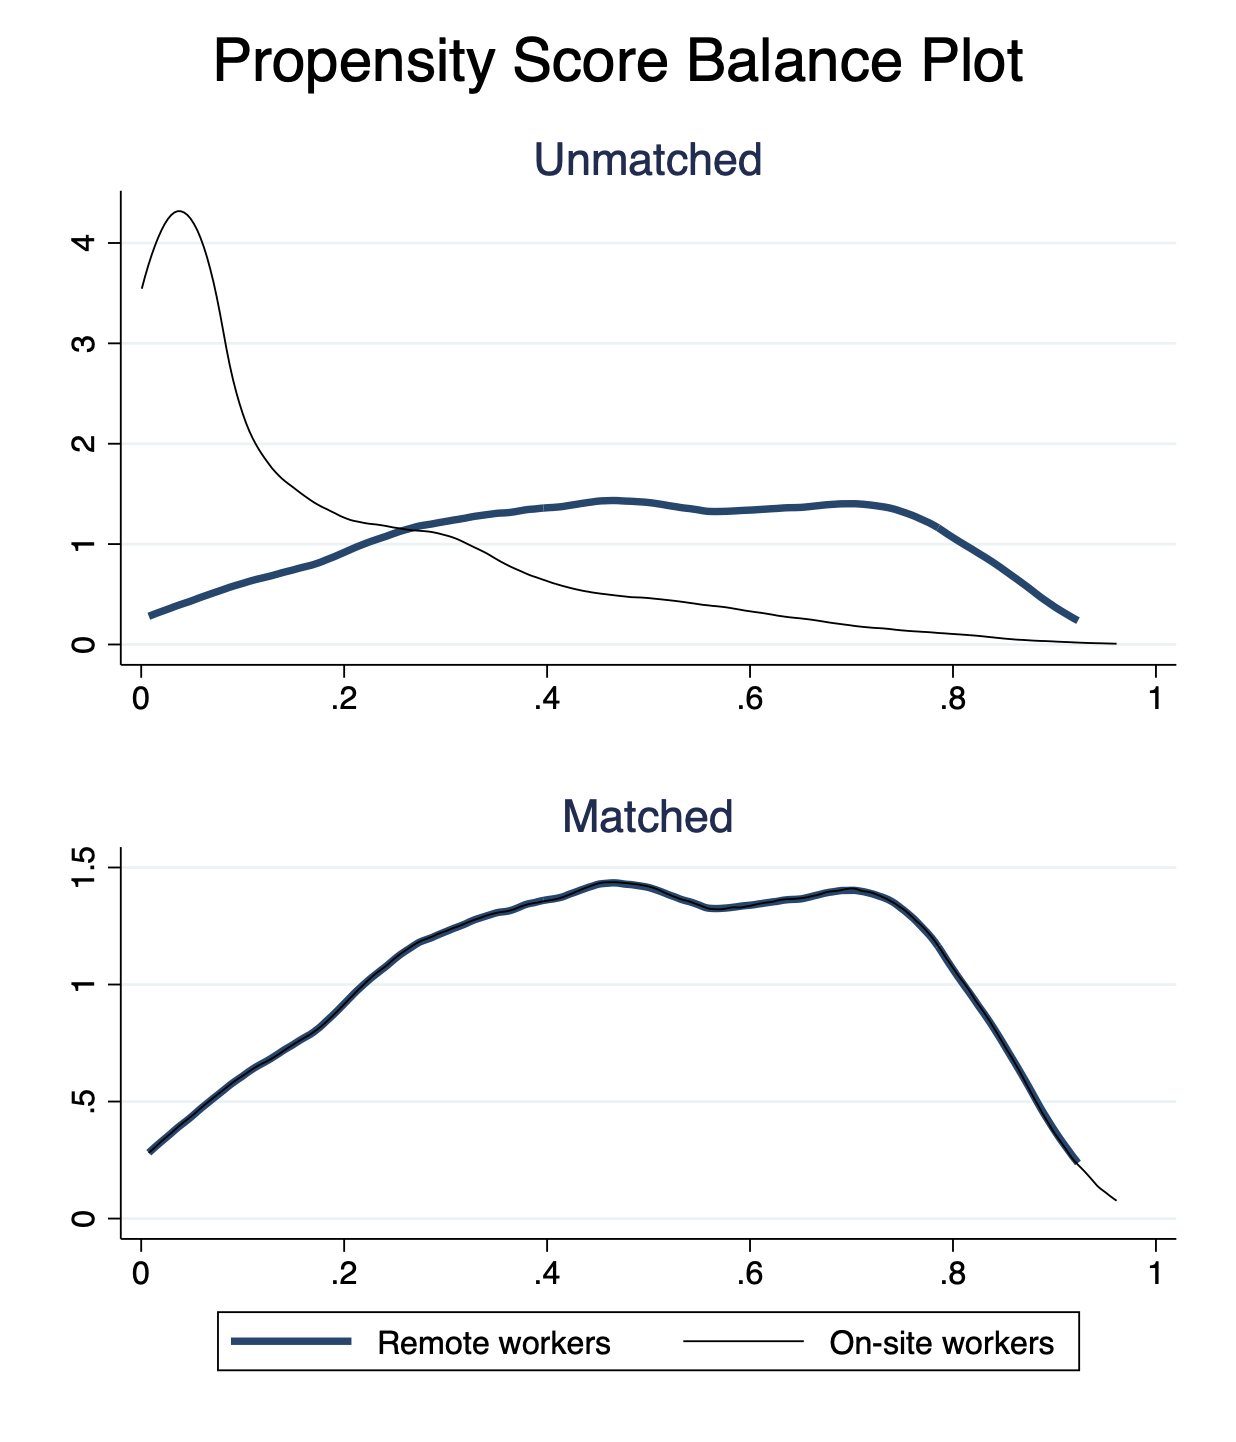
\includegraphics[width=10cm]{ps_den.png}  % both png, jpg can be used for graphs
\end{center}
\end{figure}
\vspace{-3em}

\begin{singlespace}
        \begin{footnotesize}
        		\noindent {\it Notes:} This figure illustrates the distribution of propensity scores for both the treatment group (remote workers) and the control group (on-site workers). It shows the propensity scores on the x-axis, with the fraction of observations on the y-axis. The propensity scores were calculated using a logit regression model that took into account factors such as age, sex, occupation, earnings, marital status, presence of children in the household, and state of residence. The propensity scores offer an indication of the probability that a given worker would be in the treatment group, given their specific characteristics.
        \end{footnotesize}
\end{singlespace}




\end{document}